\documentclass[12pt]{article}

\usepackage[utf8]{inputenc}
\usepackage[T1]{fontenc}
\usepackage[spanish]{babel}
\usepackage{geometry}
\geometry{letterpaper, margin=2cm}
\usepackage{graphicx}
\usepackage{float}
\usepackage{booktabs}
\usepackage{array}
\usepackage{caption}
\usepackage{subcaption}
\usepackage{hyperref}
\hypersetup{colorlinks=true, linkcolor=blue, urlcolor=blue}
\usepackage{eso-pic}
\usepackage{tikz}

\graphicspath{{figs/}}
\setlength{\parindent}{0pt}
\setlength{\parskip}{6pt}

\title{\textbf{Práctica 1. Unidad Aritmética Lógica (ALU) Simple de 4 bits}\\
\large Arquitecturas Computacionales}
\author{Robbie Nicolás Curioso de Salazar (ID 186028)\\
\textit{Hector López Sanchez (ID 185979)}\\
Universidad de las Américas Puebla\\
Profesor: Berenice Rodriguez Pedroza}
\date{\today}

\begin{document}

\AddToShipoutPictureBG{%
  \begin{tikzpicture}[remember picture,overlay]
    \node[opacity=0.08, rotate=12, anchor=south east] at ([xshift=1.8cm,yshift=-1.6cm]current page.south east)
    {
\includegraphics[width=0.72\paperwidth]{udlap_logo.png}};
  \end{tikzpicture}
}

\twocolumn[
\maketitle
\vspace{-0.5cm}
]

\section*{Objetivo}
Diseñar, sintetizar y probar en FPGA una ALU simple de 4 bits para ejecutar operaciones aritméticas y lógicas entre dos operandos de entrada. La práctica se enfocó en validar el funcionamiento del diseño tanto en Vivado como en montaje físico con protoboard.

\section*{Especificación solicitada}
De acuerdo con la práctica, la ALU recibe dos operandos de 4 bits ($A[3:0]$ y $B[3:0]$), una señal de control, y entrega un resultado de 4 bits junto con una bandera de acarreo para operaciones aritméticas.

\begin{table}[H]
\centering
\caption{Operaciones pedidas en el enunciado.}
\begin{tabular}{cl}
\toprule
ALUControl & Operación \\
\midrule
000 & ADDU \\
001 & ADDS \\
010 & SUB \\
011 & AND \\
100 & OR \\
101 & XOR \\
110 & NOR \\
\bottomrule
\end{tabular}
\end{table}

\section*{Implementación realizada}
Se trabajó sobre el repositorio:
\begin{center}
\url{https://github.com/robbienicolasai/arquitectura-computacional-alu4bits}
\end{center}

Archivos principales del laboratorio:
\begin{itemize}
  \item \texttt{src/alu1\_0.vhd}
  \item \texttt{constraints/alu4bits\_pynqz1\_pmod.xdc}
\end{itemize}

El módulo de la ALU se implementó en VHDL con un proceso combinacional y una sentencia \texttt{case} para seleccionar la operación. La asignación de pines se realizó para PYNQ-Z1 (\texttt{xc7z020clg400-1}) usando PMODA y PMODB.

\section*{Montaje físico}
La validación se realizó en protoboard mediante switches para entradas y LEDs para salidas. Se conectó tierra común entre FPGA y protoboard, y se respetó lógica a 3.3V en pines PMOD.

\section*{Resultados experimentales}
A continuación se muestran los casos capturados durante la demostración. En todos los casos, la salida observada en LEDs coincide con la operación ejecutada.

\begin{table}[H]
\centering
\caption{Resumen de pruebas con evidencia fotográfica.}
\begin{tabular}{>{\raggedright\arraybackslash}p{0.22\columnwidth} >{\raggedright\arraybackslash}p{0.2\columnwidth} >{\raggedright\arraybackslash}p{0.22\columnwidth} >{\centering\arraybackslash}p{0.18\columnwidth}}
\toprule
Operación & Entradas & Resultado esperado & Validación \\
\midrule
ADD & 1 + 1 & 2 & Correcto \\
SUB & 2 - 1 & 1 & Correcto \\
AND & 1 AND 1 & 1 & Correcto \\
OR & 3 OR 1 & 3 & Correcto \\
XOR & 3 XOR 1 & 2 & Correcto \\
NOR & 3 NOR 1 & 12 (1100) & Correcto \\
\bottomrule
\end{tabular}
\end{table}

\begin{figure}[H]
\centering
\begin{subfigure}{0.48\columnwidth}
\centering
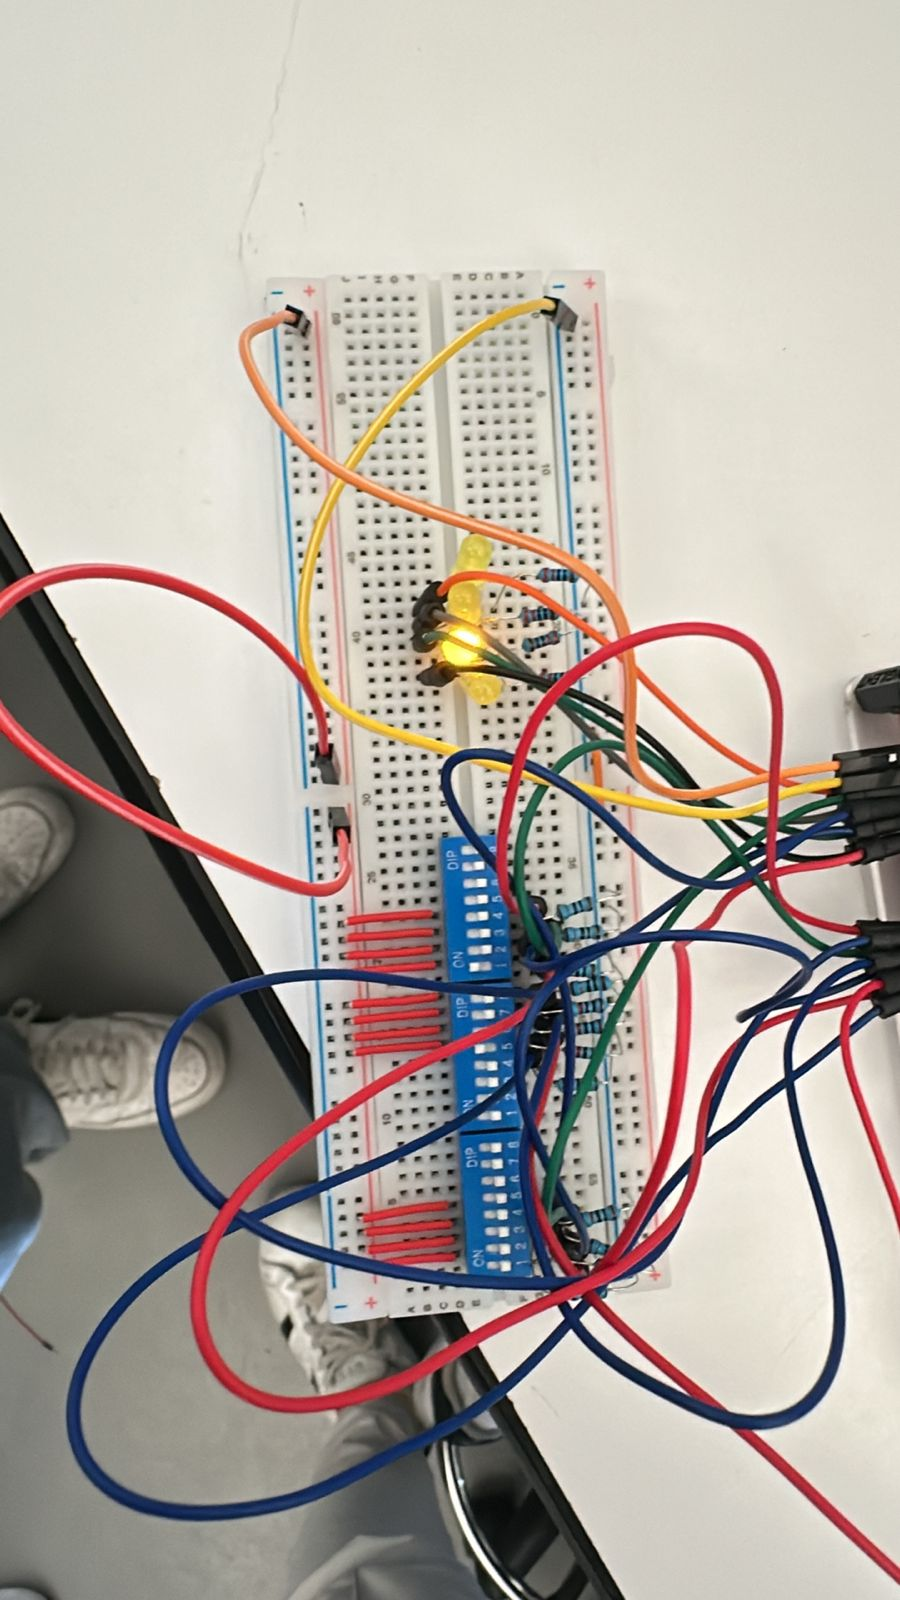
\includegraphics[width=\linewidth]{alu_add_1_1_2.jpg}
\caption{ALU\_ADD: 1 + 1 = 2}
\end{subfigure}
\hfill
\begin{subfigure}{0.48\columnwidth}
\centering
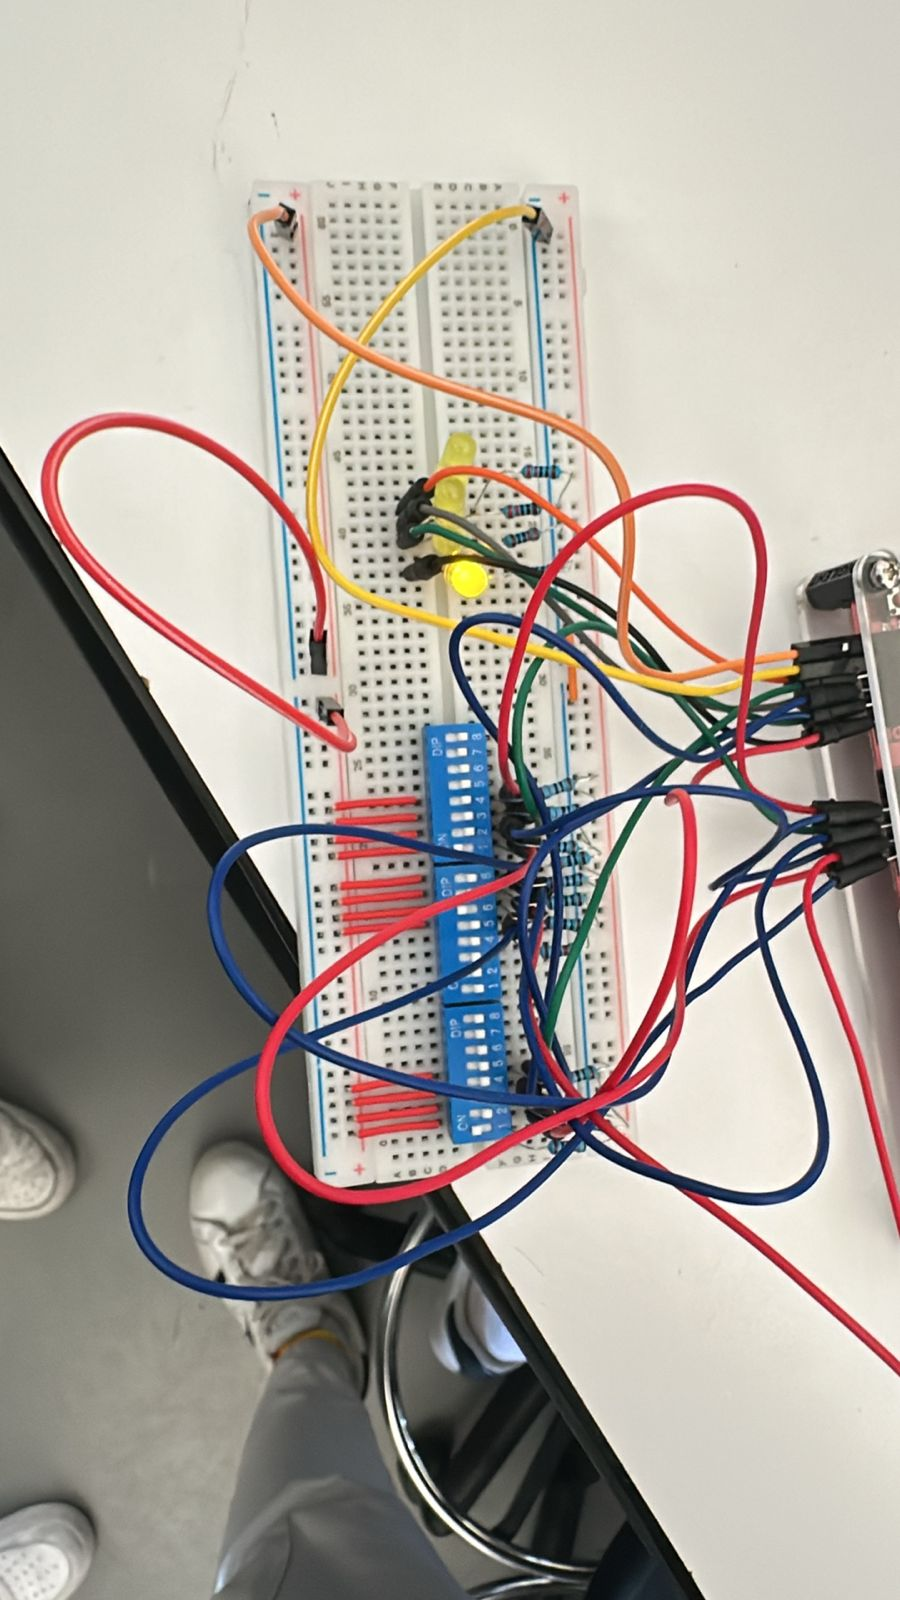
\includegraphics[width=\linewidth]{alu_sub_2_1_1.jpg}
\caption{ALU\_SUB: 2 - 1 = 1}
\end{subfigure}
\caption{Pruebas aritméticas.}
\end{figure}

\begin{figure}[H]
\centering
\begin{subfigure}{0.48\columnwidth}
\centering
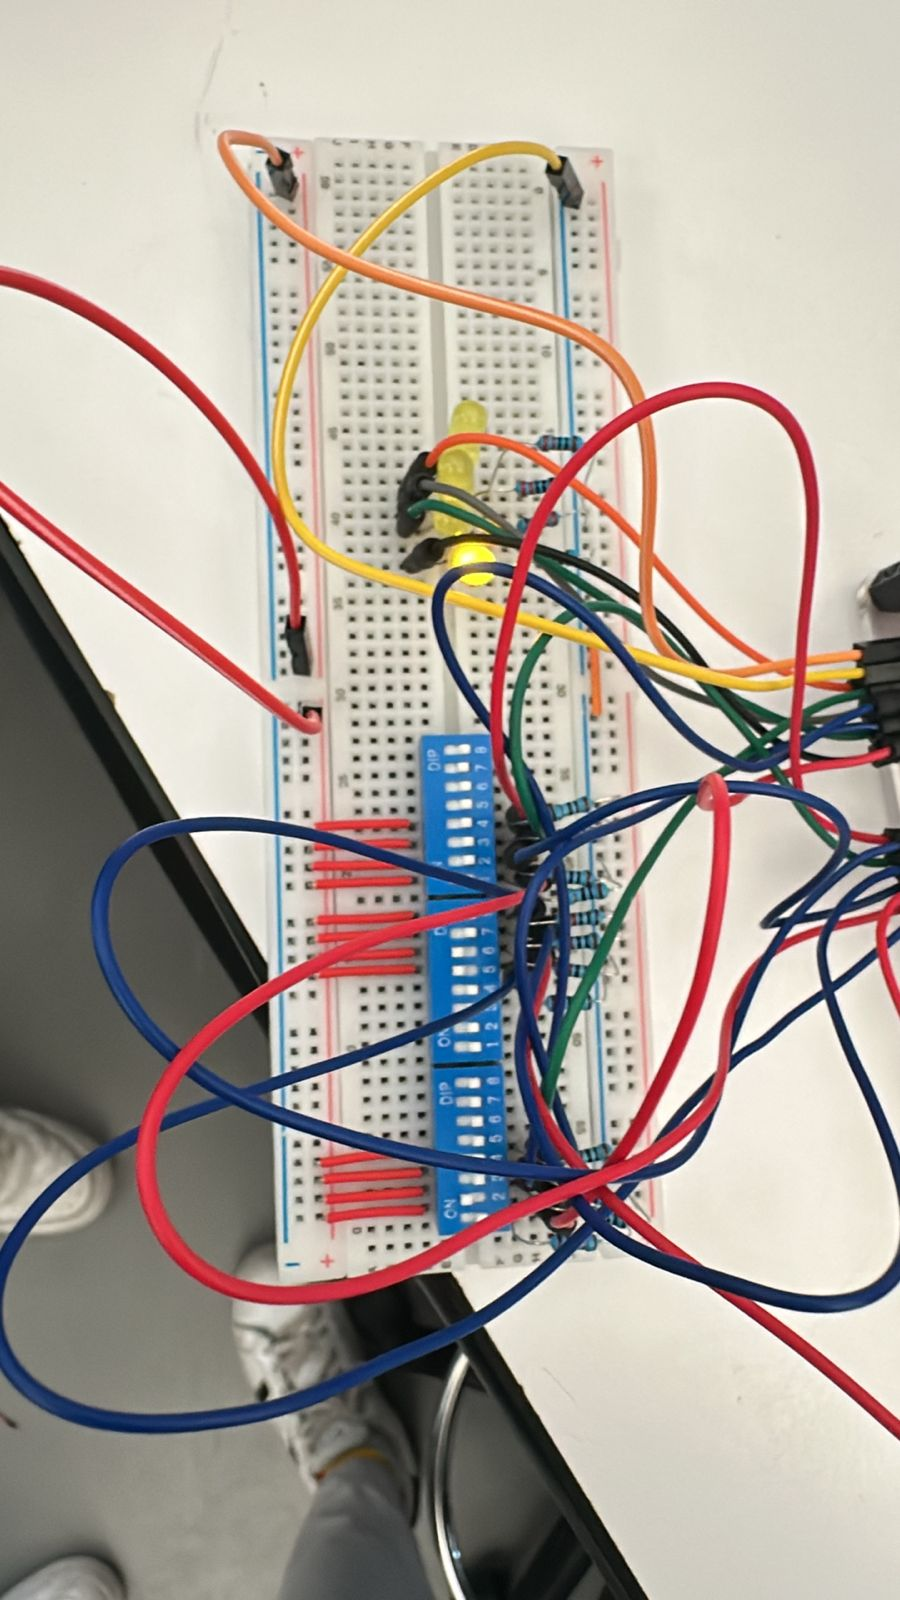
\includegraphics[width=\linewidth]{alu_and_1_1.jpg}
\caption{ALU\_AND: 1 AND 1}
\end{subfigure}
\hfill
\begin{subfigure}{0.48\columnwidth}
\centering
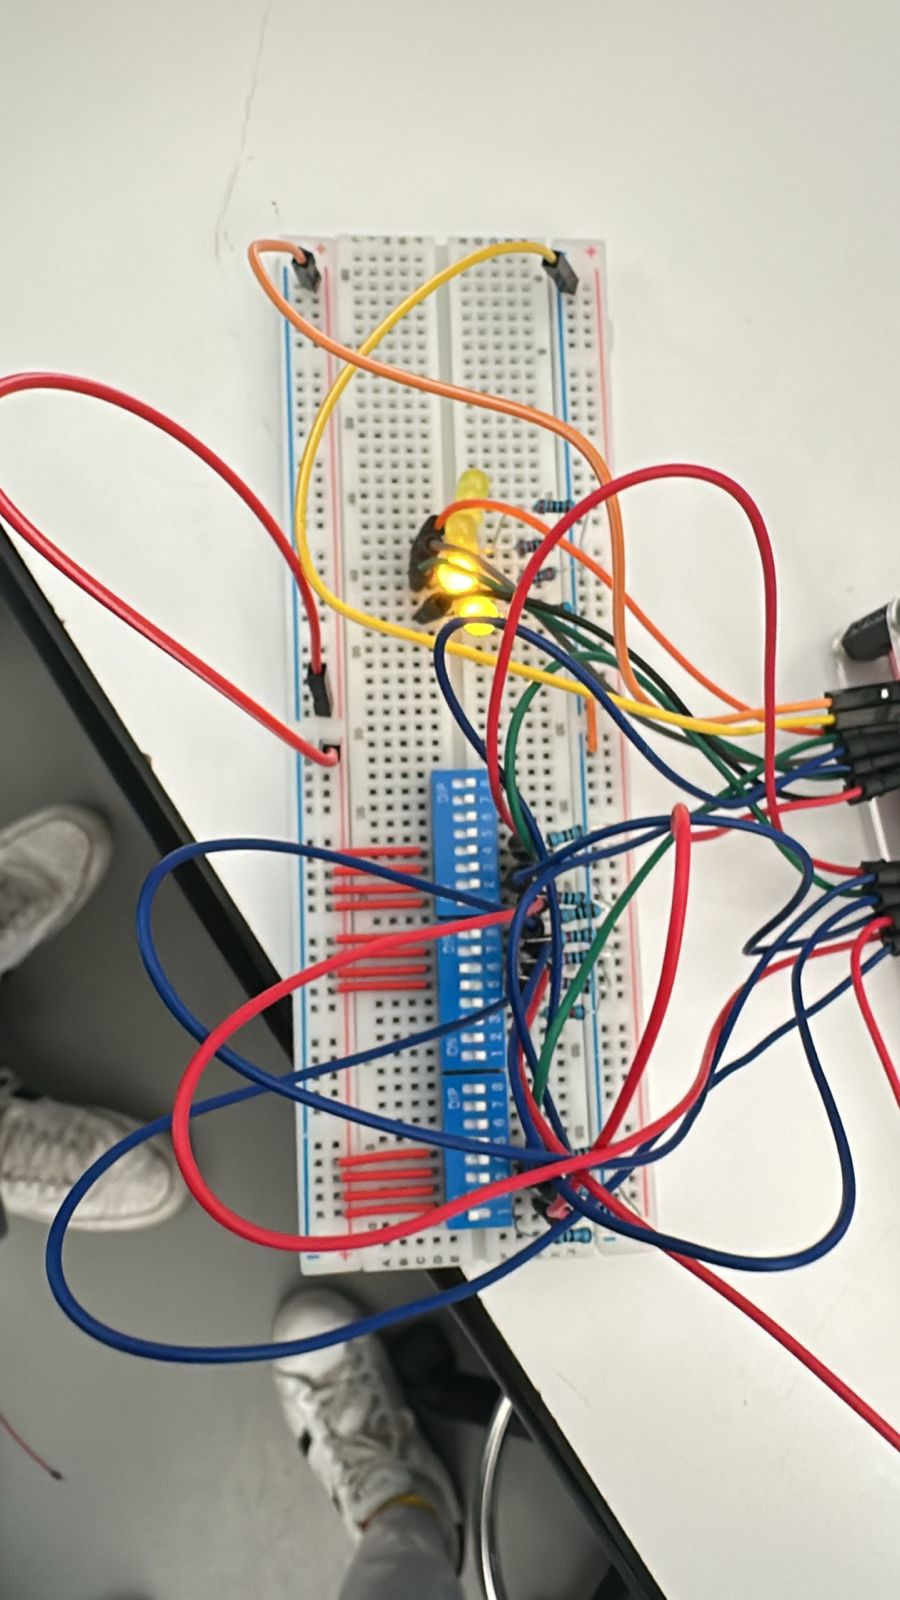
\includegraphics[width=\linewidth]{alu_or_3_1.jpg}
\caption{ALU\_OR: 3 OR 1}
\end{subfigure}
\caption{Pruebas lógicas (AND y OR).}
\end{figure}

\begin{figure}[H]
\centering
\begin{subfigure}{0.48\columnwidth}
\centering
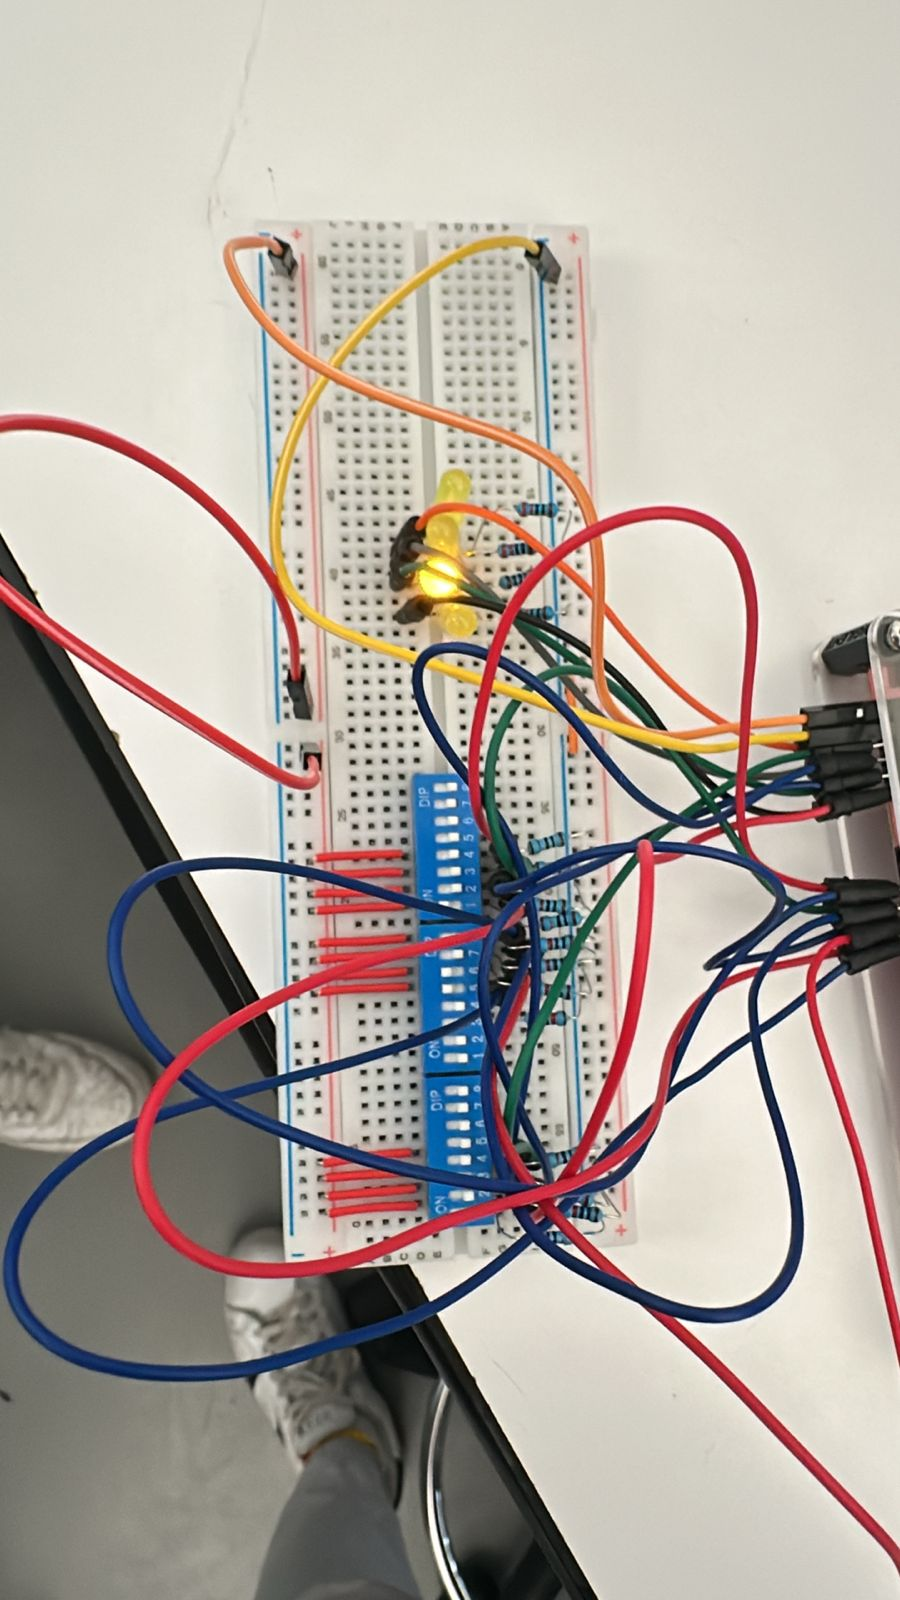
\includegraphics[width=\linewidth]{alu_xor_3_1.jpg}
\caption{ALU\_XOR: 3 XOR 1}
\end{subfigure}
\hfill
\begin{subfigure}{0.48\columnwidth}
\centering
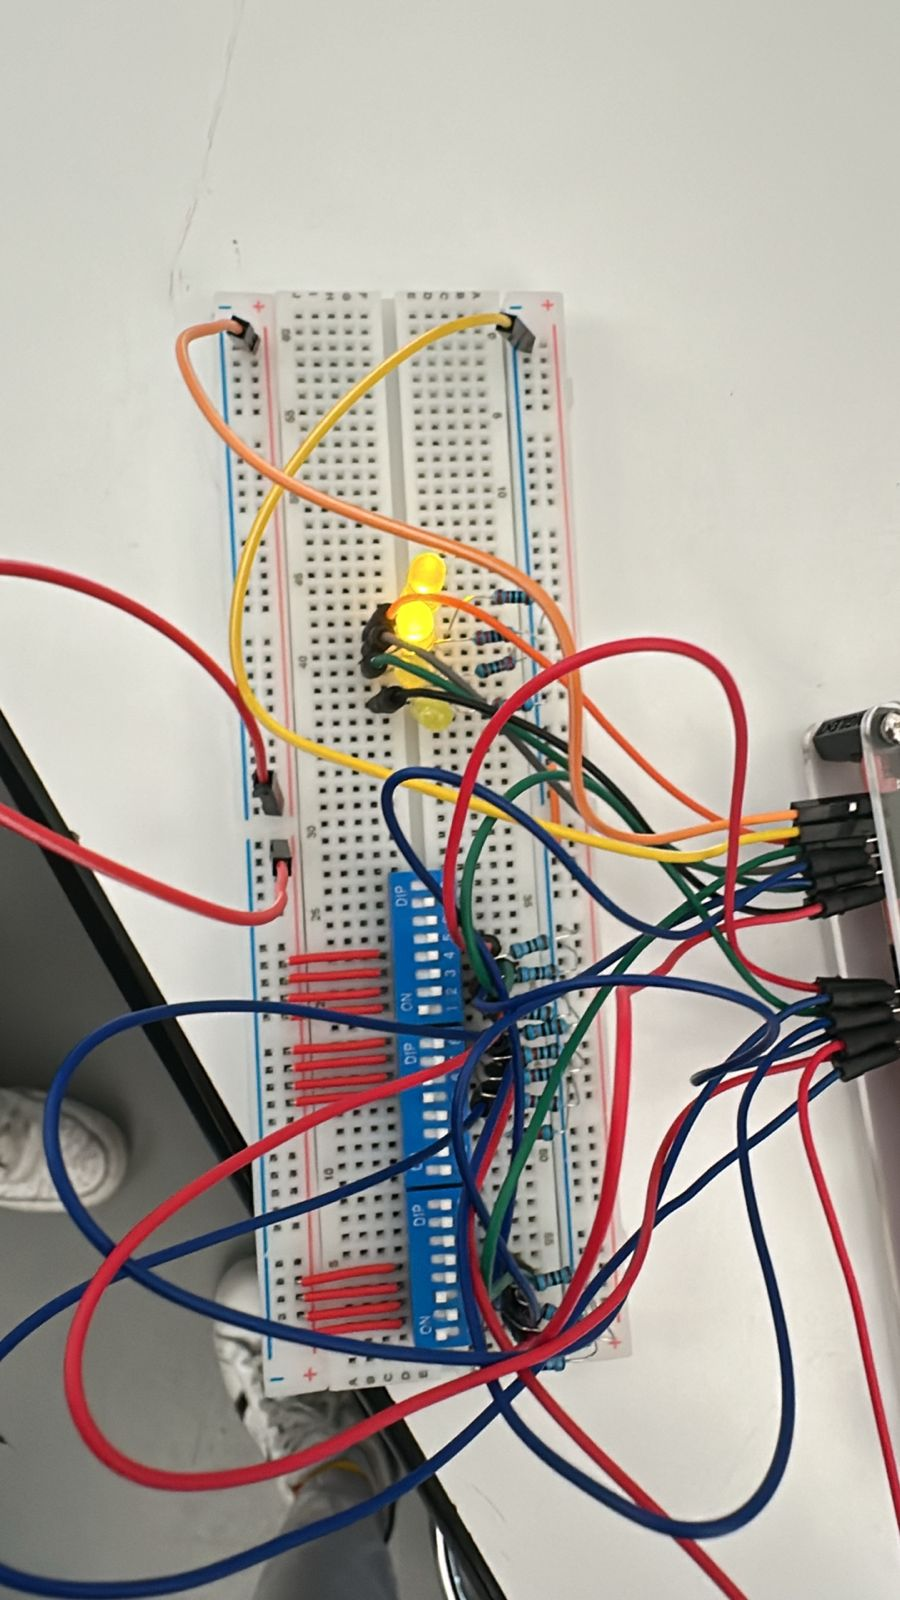
\includegraphics[width=\linewidth]{alu_nor_3_1.jpg}
\caption{ALU\_NOR: 3 NOR 1}
\end{subfigure}
\caption{Pruebas lógicas (XOR y NOR).}
\end{figure}

\section*{Discusión}
Durante la implementación, los puntos críticos fueron: (1) definir correctamente el \texttt{top module} en Vivado, (2) mantener consistencia entre nombres de puertos en VHDL y XDC, y (3) respetar el mapeo físico PMOD para evitar lecturas erróneas en la protoboard. Una vez corregidos esos puntos, el comportamiento de la ALU fue estable.

\section*{Conclusiones}
Se logró diseñar e implementar una ALU de 4 bits funcional sobre FPGA, validando operaciones aritméticas y lógicas en hardware real. La práctica reforzó el flujo completo de diseño digital: codificación en VHDL, constraints, síntesis, implementación y verificación experimental.

\section*{Referencias}
\begin{itemize}
  \item Universidad de las Américas Puebla. \textit{Práctica: Unidad Aritmética Lógica (ALU) Simple de 4 bits}.
  \item RISC-V International. \url{https://riscv.org/technical/specifications/}
  \item Repositorio del laboratorio: \url{https://github.com/robbienicolasai/arquitectura-computacional-alu4bits}
\end{itemize}

\end{document}
